%\documentclass[aps,twocolumn,secnumarabic,balancelastpage,amsmath,amssymb,nofootinbib,floatfix]{revtex4-1}

\documentclass{report}

\usepackage[colorlinks=true,linkcolor=blue]{hyperref}

% \usepackage{mathexam}
% \usepackage{booktabs}

% \usepackage{a4wide}
\usepackage[utf8]{inputenc}
\usepackage{amsmath}
\usepackage{amsfonts}
\usepackage{amssymb}
\usepackage{mathtools}
\usepackage[brazil]{babel}
%quebra de linha do sumário
%\usepackage[breaklinks=true]{hyperref}
%\usepackage{braket}
\usepackage{minitoc}
\usepackage{wrapfig}
\usepackage{subfigure}
\usepackage{setspace}
\usepackage{underscore}
\usepackage{indentfirst}
\usepackage{physics}

\usepackage{accents}

\usepackage{blindtext}

\usepackage{graphicx}
\usepackage{tikz}
\usetikzlibrary{shapes,arrows}

\usepackage{listings}
\usepackage{color}

\definecolor{mygreen}{rgb}{0,0.6,0}
\definecolor{mygray}{rgb}{0.85,0.85,0.85}
\definecolor{mymauve}{rgb}{1,0.502,0}
\definecolor{numGray}{rgb}{0.3,0.3,0.3}

\lstset{language=C,
  backgroundcolor=\color{mygray},   % choose the background color; you must add \usepackage{color} or \usepackage{xcolor}; should come as last argument
  basicstyle=\footnotesize,        % the size of the fonts that are used for the code
  breakatwhitespace=false,         % sets if automatic breaks should only happen at whitespace
  breaklines=true,                 % sets automatic line breaking
  captionpos=b,                    % sets the caption-position to bottom
  commentstyle=\color{mygreen},    % comment style
  deletekeywords={...},            % if you want to delete keywords from the given language
  escapeinside={\%*}{*)},          % if you want to add LaTeX within your code
  extendedchars=true,              % lets you use non-ASCII characters; for 8-bits encodings only, does not work with UTF-8
  frame=single,	                   % adds a frame around the code
  keepspaces=true,                 % keeps spaces in text, useful for keeping indentation of code (possibly needs columns=flexible)
  keywordstyle=\color{blue},       % keyword style
  language=C,                 % the language of the code
  morekeywords={*,...},            % if you want to add more keywords to the set
  numbers=left,                    % where to put the line-numbers; possible values are (none, left, right)
  numbersep=5pt,                   % how far the line-numbers are from the code
  numberstyle=\tiny\color{numGray}, % the style that is used for the line-numbers
  rulecolor=\color{black},         % if not set, the frame-color may be changed on line-breaks within not-black text (e.g. comments (green here))
  showspaces=false,                % show spaces everywhere adding particular underscores; it overrides 'showstringspaces'
  showstringspaces=false,          % underline spaces within strings only
  showtabs=false,                  % show tabs within strings adding particular underscores
  stepnumber=1,                    % the step between two line-numbers. If it's 1, each line will be numbered
  stringstyle=\color{mymauve},     % string literal style
  tabsize=2,	                   % sets default tabsize to 2 spaces
  title=\lstname                   % show the filename of files included with \lstinputlisting; also try caption instead of title
}




\onehalfspacing


\newcommand*{\dt}[1]{%
  \accentset{\mbox{\large\bfseries .}}{#1}}
\newcommand*{\ddt}[1]{%
  \accentset{\mbox{\large\bfseries .\hspace{-0.25ex}.}}{#1}}
\newcommand*{\dddt}[1]{%
  \accentset{\mbox{\large\bfseries .\hspace{-0.25ex}.\hspace{-.20ex}}}{#1}}
\newcommand*{\dnt}[2][4]{\dt{#2}^{\tiny(#1)}}
\newcommand{\esimo}{-\text{ésimo}}
\newcommand{\esima}{-\text{ésima}}

\makeatletter
\newcommand*{\gnuplotinput}[2][1.0]{%
  \begingroup
  \let\@gnplt@input@includegraphics=\includegraphics
  \def\includegraphics##1{\@gnplt@input@includegraphics[scale=#1]{#2}}%
  \let\@gnplt@input@picture=\picture
  \def\picture{\unitlength=#1\unitlength\relax\@gnplt@input@picture}%
  \input{#2}%
  \endgroup
}
\makeatother

\newcommand{\PraticeQuestion}[2]{
  \begin{center}
    \LARGE \textbf{Física Computacional - Prática #1} \\
    \Large \textbf{Questão #2} \\
    \large Alex Enrique Crispim
  \end{center}
}



\begin{document}
  \PraticeQuestion{9}{4}

  O método FTCS (\textit{foward-time centered-space}) consiste numa forma de se transformar uma equação diferencial partial dependente de uma variável denotada tempo ($t$) e uma outra  variável, a qual vamos chamar posição\footnote{A generalização para mais outra variáveis "espaciais" é feita trivialmente, trocando-se $\pdv{x}$ por $\grad$.}

  Seja
  \begin{equation}
    \pdv{T}{t} = f(T(t,x), \pdv*[2]{T}{x}, t, x)
  \end{equation}
  a equação que desejamos resolver. Comecemos por truncar a série de Taylor em primeira ordem, de forma a trocar $\pdv*[2]{T}{x}$ por
  \begin{equation*}
    \pdv[2]{T}{x} (t, x) = \frac{T(t, x-a) + T(t, x+a) - 2T(t,x)}{a^2}.
  \end{equation*}

  Para cada $x$ fixo, temos
  \begin{equation*}
    \pdv{T}{t} (t,x) = f(T(t,x), T(t, x-a), T(t, x+a), t, x).
  \end{equation*}

  Da forma como temos a equação acima, para cada $x$, $t$ varia de forma independete de $x$, de tal forma que podemos identificar a derivada parcial com relação ao tempo com a derivada total. Estamos, então, na presença de uma equação diferencial ordinária (EDO). Podemos fazer uso dos métodos já conhecidos para a solução de EDO's.

  Como truncamos a série em primeira ordem, nosso erro no cálculo de $\pdv*[2]{T}{x}$ é de segunda ordem, de forma que utilizarmos um método com erro de terceira ordem ou mais (RK2 ou RK4, por exemplo), não nos dará melhores resultados que um método cujo erro é de primeira ordem (Euler, por exemplo, cujo truncamente ocorre em primeira ordem também).

  A seguir apresentamos o resultado obtido para algumas temperaturas. O programa feito (disponível em \url{https://github.com/AlexEnrique/pratice-9-and-10}) fora feito de forma diferente do pedido pelo exercício. Explicaremos o motivo de tal escolha.

  \newpage
  Ao construir o programa, fizemos uso da técnica de \textit{passagem de argumentos via linha de comando}. Basicamente, passamos argumento para o programa diretamente na hora de chamá-lo, escrevendo-os logo após o comando de execução do programa. Por exemplo, digitar \texttt{./programa.x 3.12 22 a} chama o programa de nome \texttt{programa.x}, passando os argumentos \texttt{3.12, 22} e \texttt{a} para o programa. Tais argumentos são lidos e podem ser utilizados pelo programa da forma como se desejar.

  Para fazermos isso, definimos a função \texttt{main} da seguinte forma
  \begin{lstlisting}
    int main (int argc, char *argv[]);
  \end{lstlisting}
  A variável \texttt{argc} é responsável por contar o número de parâmetros passados via linha de comando, somado a 1. Esse 1 a mais se refere a própria chamada do programa. Os parâmetros passados são armazenados como um tipo \texttt{char *} no array \texttt{argv[]}. O primeiro elemento deste array, \texttt{argv[0]} guarda a chamada do programa (para o exemplo anterior, \texttt{argv[0] == ./programa.x}). Os demais elementos são armazenados na ordem em que foram passados.
  Interessante citar a opção de se utilizar as funções \texttt{atoi()} e \texttt{atof()} (e outras) da biblioteca \texttt{<string.h>} para converter tipos \texttt{char *} em inteiros e pontos flutuantes (dupla precisão), o que nos dá maiores opções para a passagem de parâmetros via linha de comando.

  Escolheu-se aceitar 3 parâmetros: o tempo final (denominado \texttt{tEnd}), uma opção de plotagem (\texttt{<plot option>}) e o nome do arquivo de (dados de) saída (\texttt{<file name>}). Requer-se que, pelo menos o parâmetro de tempo final seja passado. Com efeito, se não se passa tal parâmetro, a seguinte mensagem de erro é impressa na tela:
  \begin{figure}[h]
    \center
    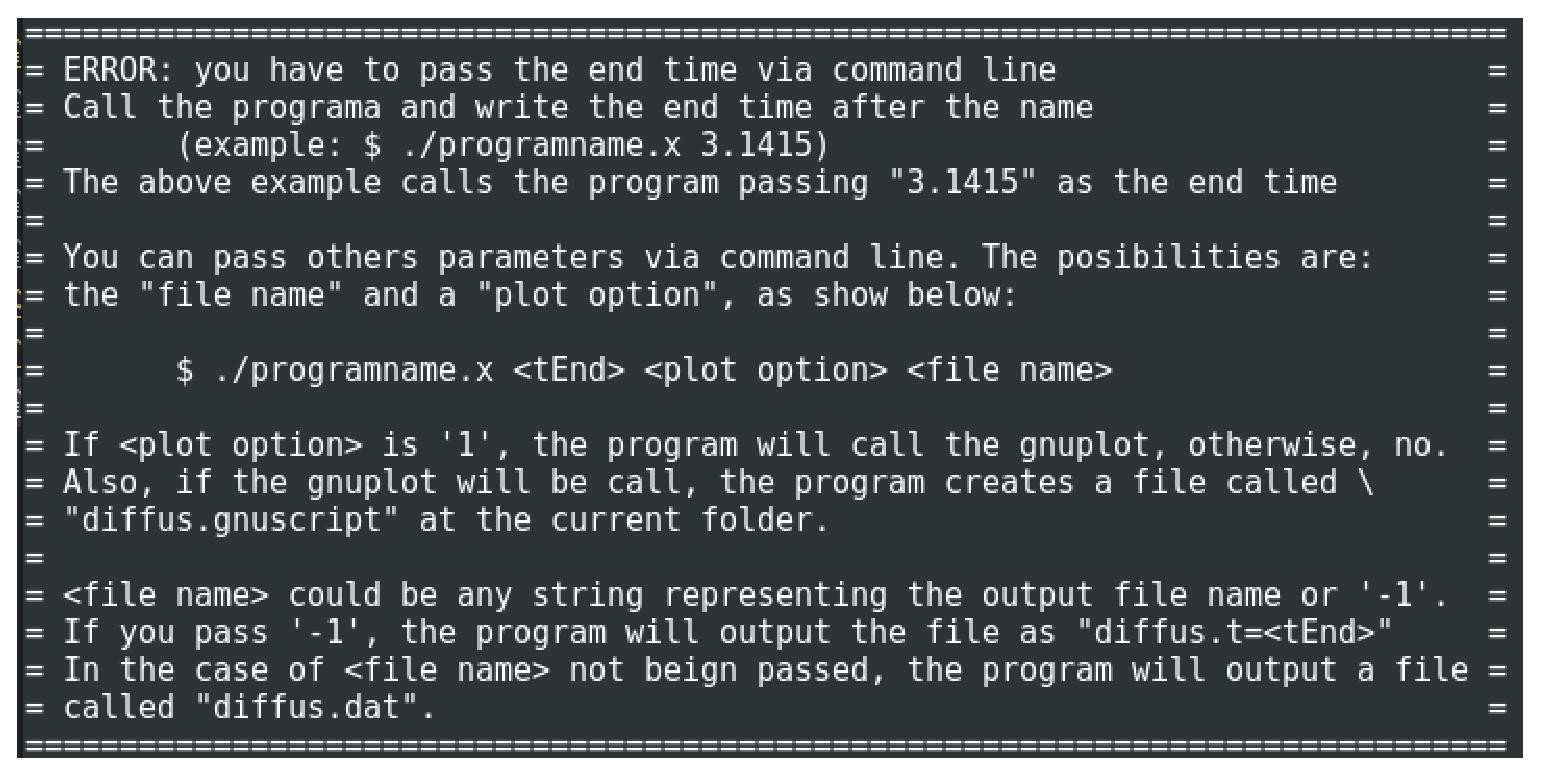
\includegraphics[scale = .35]{outputq4}
  \end{figure}


  \newpage
  Optou-se por fazer uso de tal método na criação do programa de forma a fazer um programa de uso mais amplo e, em certo sentido, mais simples. Para se fazer o que se pede no enunciado do exercício, bastaria criar um outro código que chamasse o mesmo programa e passasse os valores requeridos de \texttt{tEnd}. Abaixo temos um exemplo (quase que no formato de um pseudo-código).
  \begin{lstlisting}
    int main () {
      double t[] = [t1, t2, t3]; // colocar os tempos requeridos

      for (i = 0; i < t.length; i++) {
        snprintf(buffer, BUFFER_SIZE, "./program.exe %lf 0 -1", t[i]);
        system(buffer) // passa a string buffer para o terminal, como comando
      }
    }
  \end{lstlisting}

  O reaproveitamento do programa se torna maior com o uso dos argumentos da função main().

  Abaixo temos um gráfico para os três valores de tempo pedidos no enunciado.

  \begin{figure}[h]
    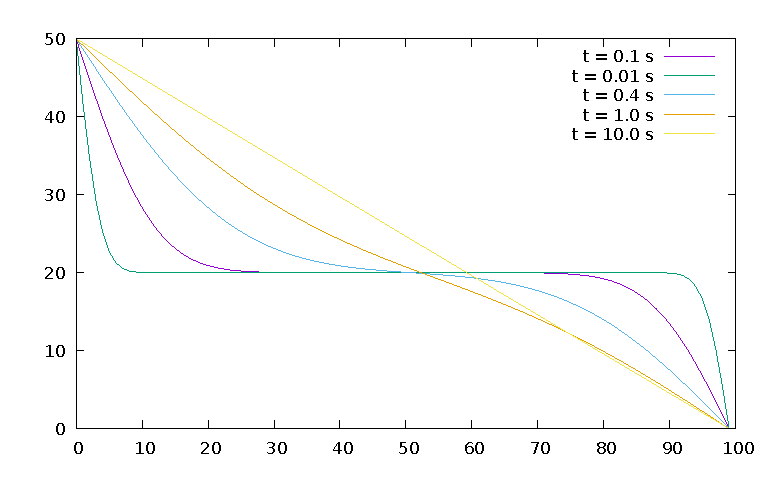
\includegraphics[scale = 1.0]{q4.eps}
    \caption{Solução para a equação de difussão}
  \end{figure}

\end{document}
